\documentclass[a4paper,11pt]{article}
\author{ 杨旭鹏  \  PB17000234}
\date{2019年秋季}
\title{计算物理A 第六题}

\usepackage{ctex}
\usepackage{amsmath}
\usepackage{amsfonts}
\usepackage{graphicx}
\usepackage{epstopdf}
\usepackage{lastpage}
\usepackage{hyperref}
\usepackage{listings}
\RequirePackage{xcolor}
\usepackage{appendix}
\usepackage{caption2}
\usepackage{subfigure}
\usepackage{float}
\makeatletter\def\@captype{table}\makeatother

\definecolor{dkgreen}{rgb}{0,0.6,0}
\definecolor{gray}{rgb}{0.5,0.5,0.5}
\definecolor{mauve}{rgb}{0.58,0,0.82}

\lstset{
  frame=tb,
  aboveskip=3mm,
  belowskip=3mm,
  showstringspaces=false,
  columns=flexible,
  framerule=1pt,
  rulecolor=\color{gray!35},
  backgroundcolor=\color{gray!5},
  basicstyle={\small\ttfamily},
  numbers=left,
  numberstyle=\tiny\color{gray},
  keywordstyle=\color{blue},
  commentstyle=\color{dkgreen},
  stringstyle=\color{mauve},
  breaklines=true,
  breakatwhitespace=true,
  tabsize=3,            
  }



\begin{document}
\maketitle

\section{题目描述}
对两个函数线型(Gauss 分布和 类Lorentz 型分布),设其一为 $p(x)$,另一为 $F(x)$,用舍选法对 $p(x)$ 抽样。将计算得到的归一化频数分布直方图与理论曲线 $p(x)$ 进行比较,讨论差异。讨论抽样效率。
\begin{equation}
	Gaussian:\sim e^{-\frac{x^{2}}{2}} ~~~~~Lorentzian ~ like:\sim \frac{1}{1+x^{4}}
\end{equation}



\section{算法}
\subsection{舍取法}
所要实现的抽样是$p(x) = \frac{1}{1+x^{4}}$,比较函数为$F(x)=1.1e^{-\frac{x^{2}}{2}}$。由于$p(x)$为峰状结构函数,故我们采取变换抽样与舍取抽样相结合的方式来提高抽样效率。我们有:

\begin{figure}[!htbp]        
\centering
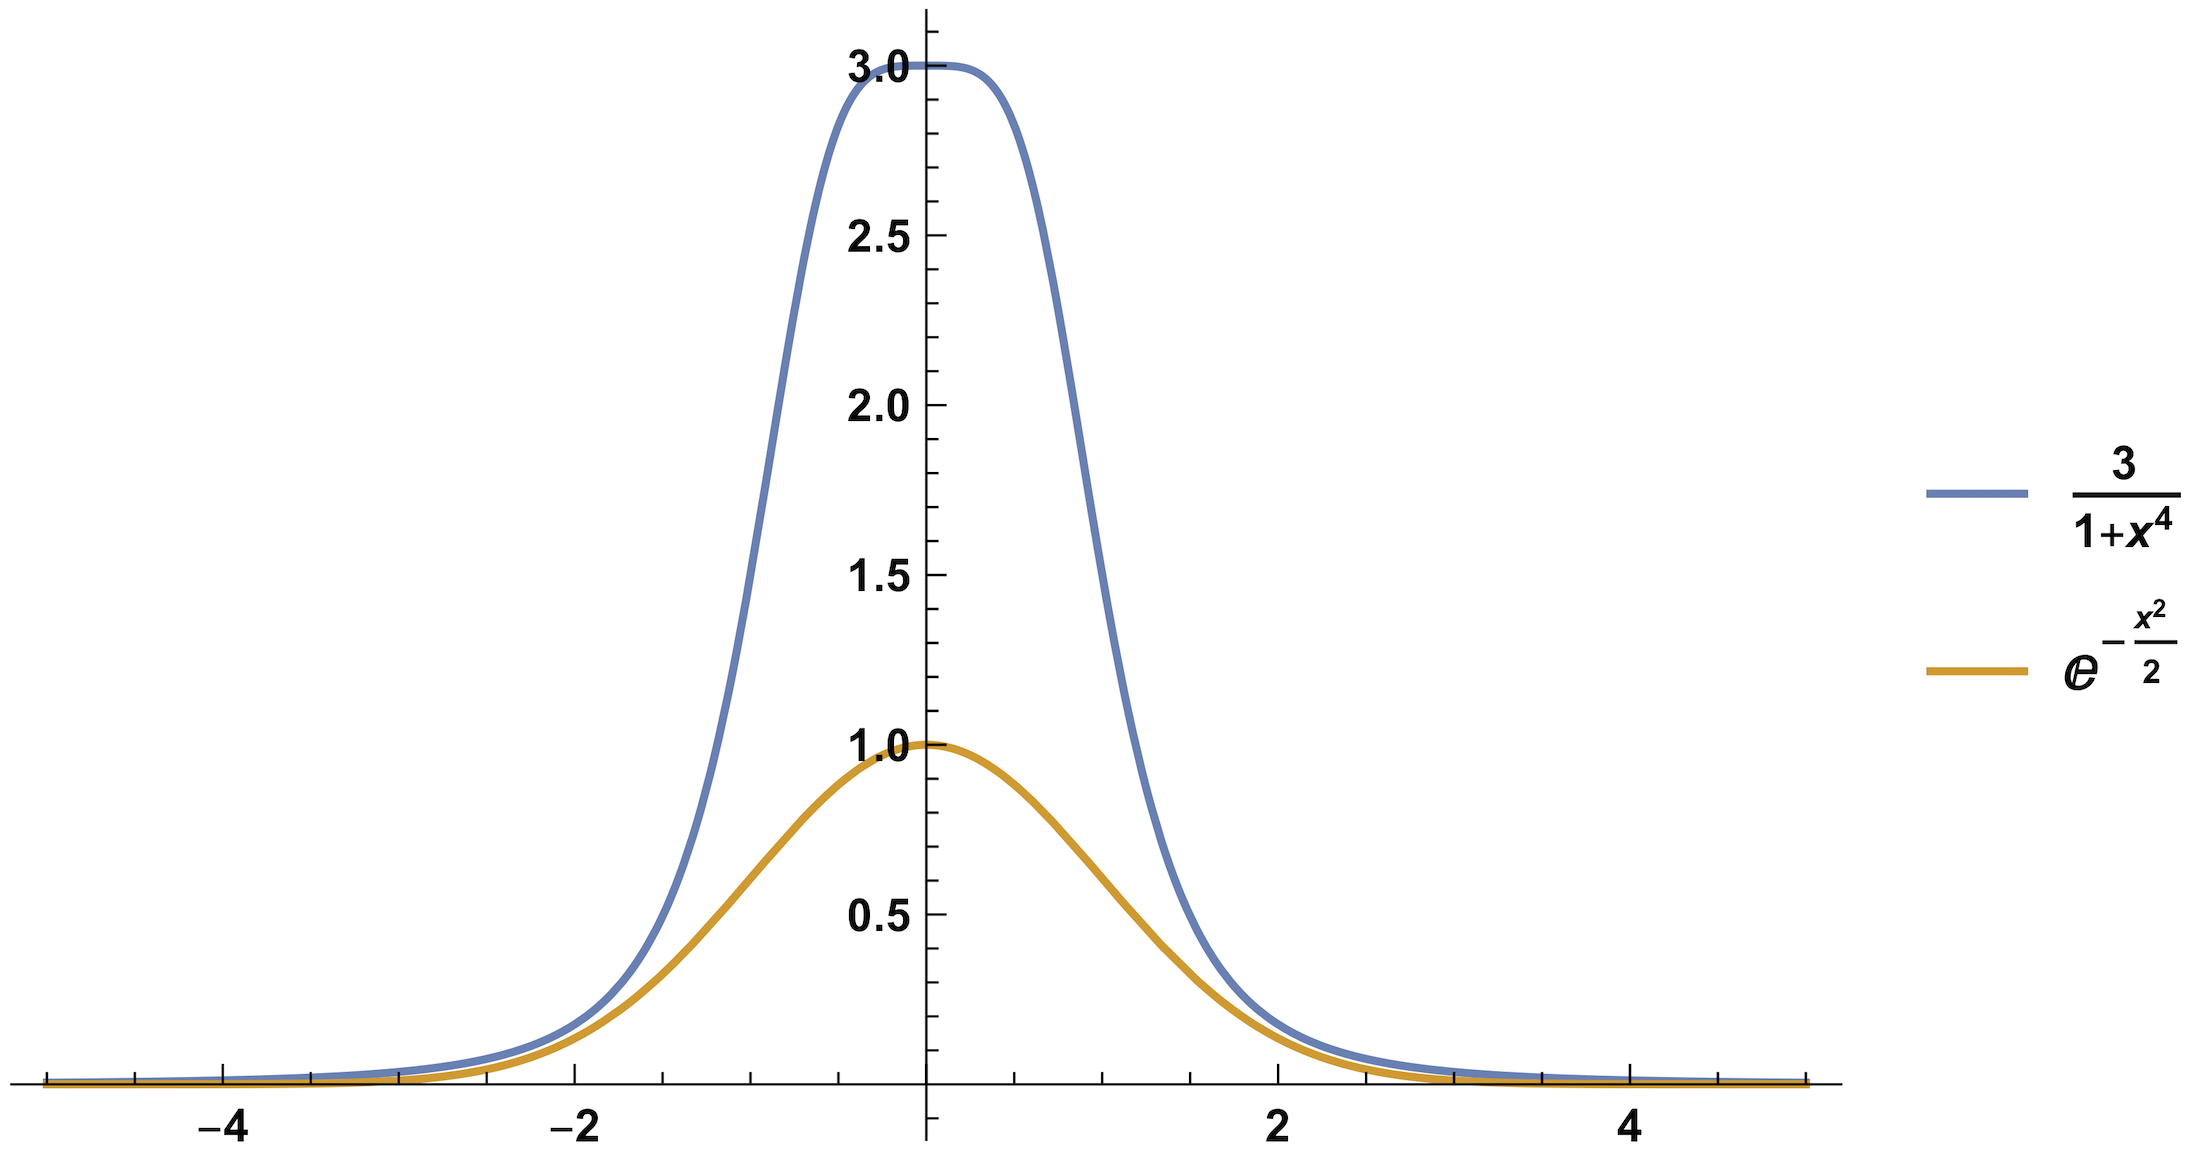
\includegraphics[width=10cm]{1.png}      
\caption{ $p(x)$与$F(x)$}      
\end{figure}

\begin{figure}[!htbp]        
\centering
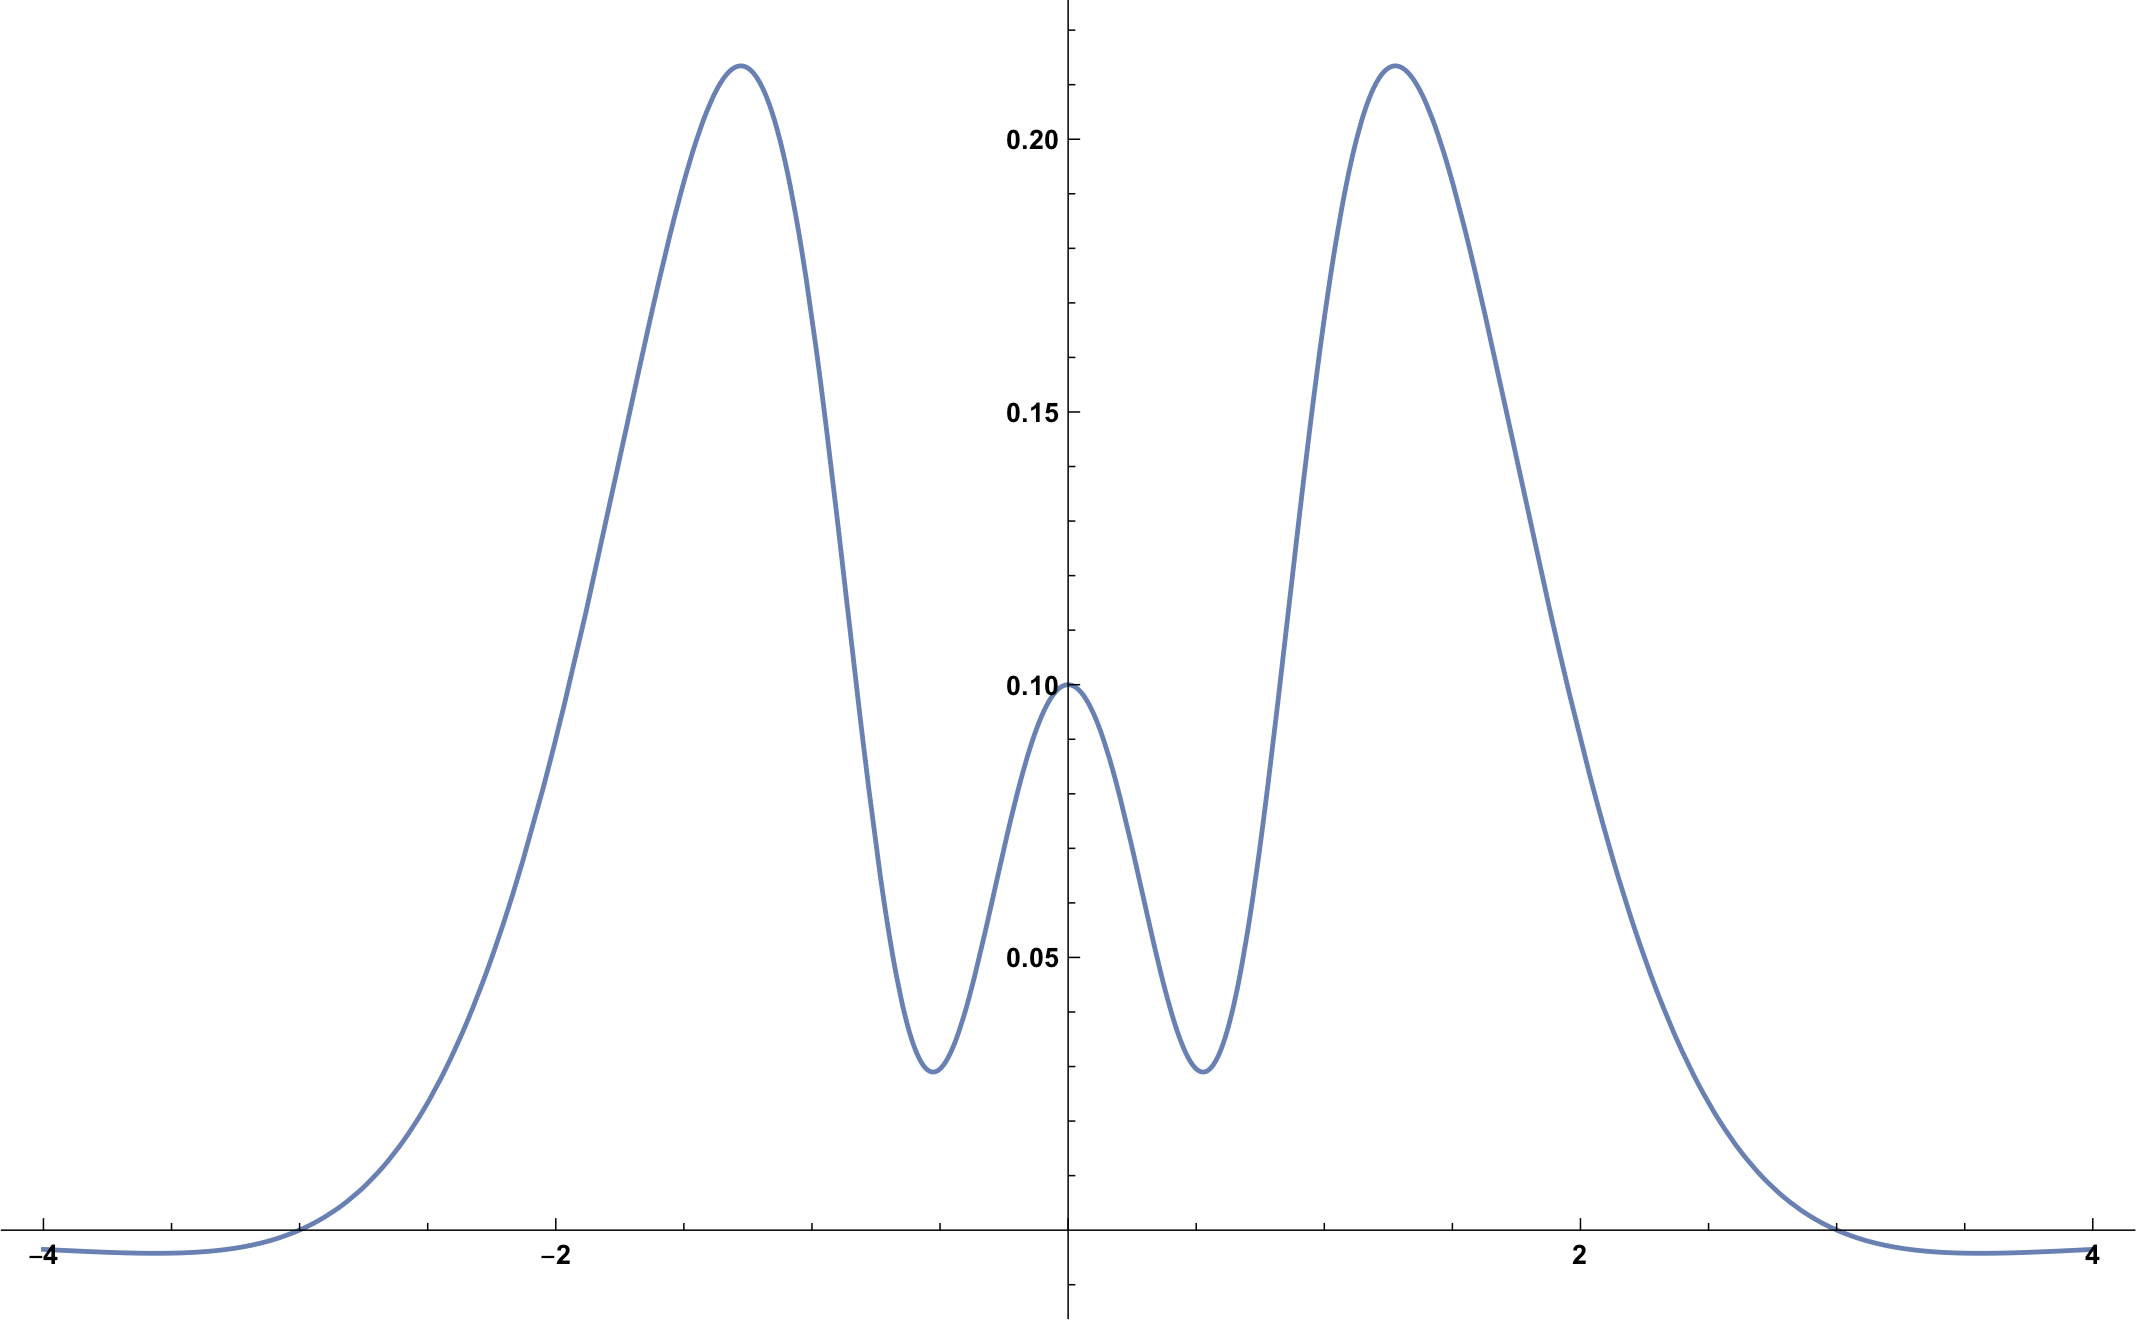
\includegraphics[width=10cm]{2.png}     
\caption{ $F(x)-p(x)$}      
\end{figure}


对$F(x)$,其为高斯分布,我们可选定对其$3\sigma$区间即$x \in [-3,3]$抽样。在此区间满足$F(x)>p(x)$($F(3)-p(3)\doteq 0.0000247742 > 0$),于是可采取变换抽样与舍取抽样相结合的方式对$p(x)$进行抽样。对于其中的高斯函数部分,我们可以利用Box-Muller 法进行抽样。而Box-Muller 法的实现方法为:
\begin{description} 
\item[1] 随机抽样一对均匀分布的随机数,$ u  \in [ 0,1 ],v \in [0,2\pi]$ ;
\item[2] 令$x=\sqrt{-2lnu}cosv$
\end{description}

则得到概率密度函数$c~e^{-\frac{x^{2}}{2}}$的抽样。(其中$c$为一正常数,由于概率密度函数的绝对大小没有意义,只有相对大小有意义,故同样的抽样方法可对应相差为正常数倍的概率密度函数。)
再在$[0,1]$均匀抽取抽取点$\eta$,则判断$F(x)\eta$是否小于等于$p(x)$,若小于,则取此$x$值,若不是,则舍。


\subsection{16807产生器}
16807产生器属于线性同余法产生器的特例。而线性同余法方法为:

\begin{equation}
\begin{aligned}
	I_{n+1} &= (aI_{n} + b) \ mod \ m \\
	x_{n} &= I_{n}/m
\end{aligned}
\label{linear}	
\end{equation}

其中整数$I_{i} \in [0,m-1]$,$a,b,m$为算法中的可调参数,其选取直接影响产生器的质量。选取参数:
\begin{equation}
\left\{
\begin{array}{l}
	a = 7^{5} = 16807 \\
	b = 0 \\
	m = 2^{31}-1 = 2147483647
\end{array}
\right.
\end{equation}

即为所谓的16807产生器。由于直接利用\ref{linear}编写程序时计算$(aI_{n} \ mod \ m )$时很容易造成数据溢出,故采取Schrage方法进行具体编程的实现:

\begin{equation}
	aI_{n} \ mod \ m = \left\{
	\begin{array}{l}
		a(I_{n}\ mod \ q) - r[I_{n}/q],\ \ \ \ \ \ \ \ if \geq 0 \\
		a(I_{n}\ mod \ q) - r[I_{n}/q] + m,\ \ otherwise	
			\end{array}
	\right.
\end{equation}

其中$m=aq+r$,即$q=m/a=127773$,$r=m \ mod \ a=2836$。即可利用此方法产生伪随机数序列。



\section{程序使用方法}
在运行程序后,会看到请求输入所需总随机点数的提示,按照提示在后面输入所需要的总随机点数,摁回车继续。然后经过计算在屏幕上给出舍选法的抽样效率并统计在$[-3,3]$上剖分的$o$个小区间上抽样点出现的概率到数据文件。程序输出完这些后会自动退出。
\begin{figure}[!htbp]        
\centering

\includegraphics[width=7cm]{example.png}      
\caption{ 一个典型程序的运行示例}      
\end{figure}


\newpage
\section{程序结果与讨论}
当输入一些不同的点数时,得到如下结果\footnote{以下的结果是将$[-3,3]$剖分为600个小区间得到的(即每个小区间的长度为$0.01$)其中概率为在$[-3,3]$之间归一化后的结果,例如对于在$[x_{i},x_{i+1}]$中出现的概率,对于抽样点来说即为:$p_{i} = \frac{n_{i}}{N}$($n_{i}$为在此区间内抽样得到的点数,$N$为抽样总点数);对于理论频率来说,即为:$p_{i} = \frac{ \int_{x_{i}}^{x_{i+1}}p(x)dx }{ \int_{-3}^{3}p(x)dx } \doteq \frac{ p(\frac{x_{2}+x_{i+1}}{2})\Delta x }{ \int_{-3}^{3}p(x)dx }$(其中$\Delta x$为区间长度)}:

\begin{figure}[!htbp]        
\centering
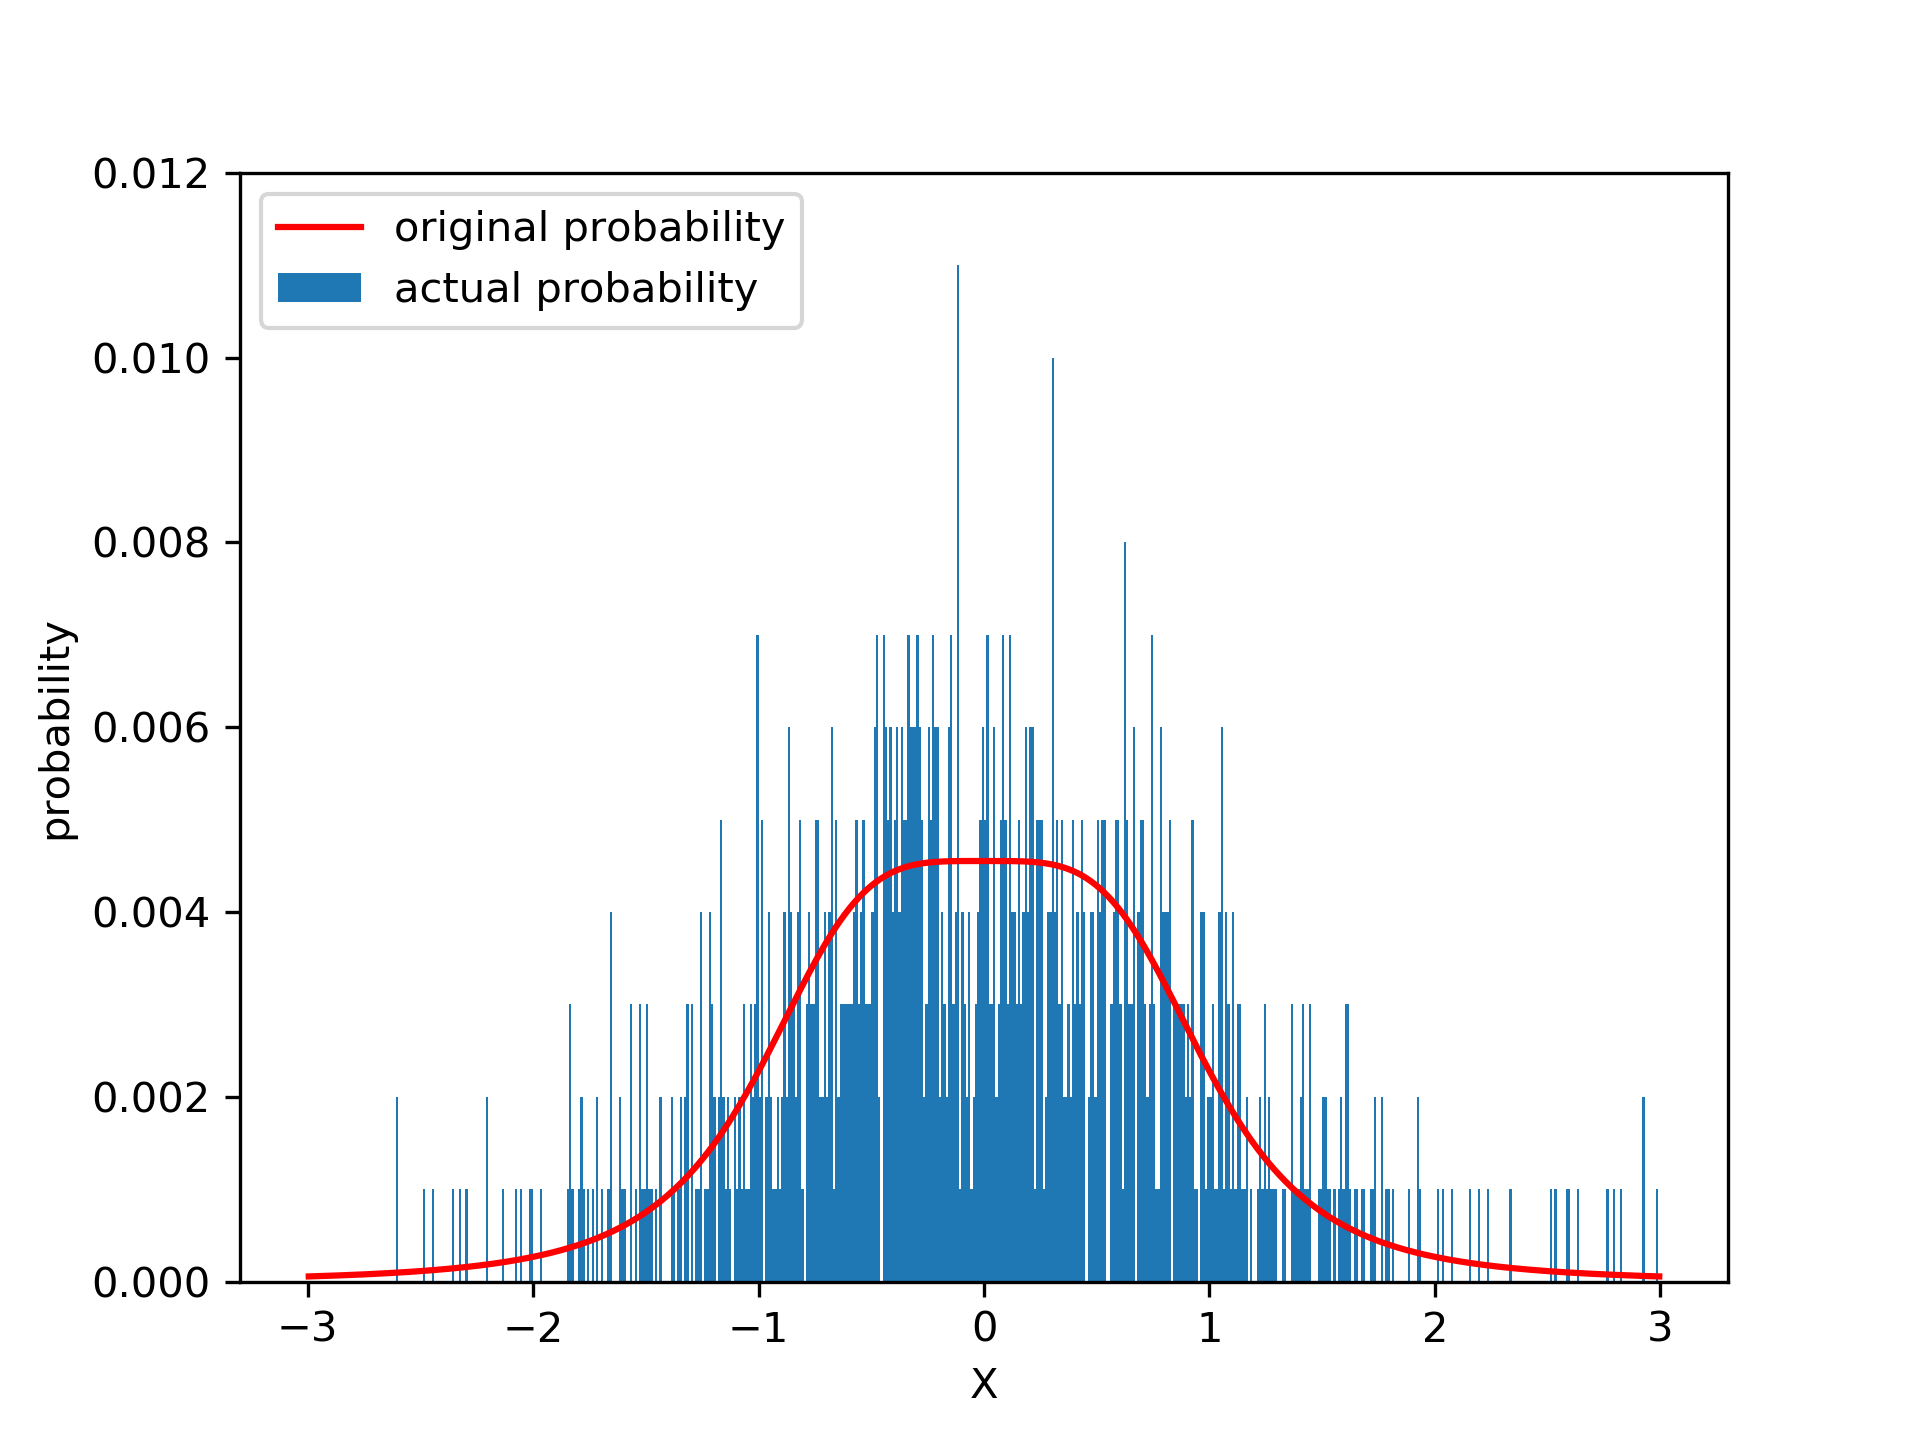
\includegraphics[width=10cm]{103.png}      
\caption{ 产生$10^{3}$个点时的结果}      
\end{figure}

\begin{figure}[!htbp]        
\centering
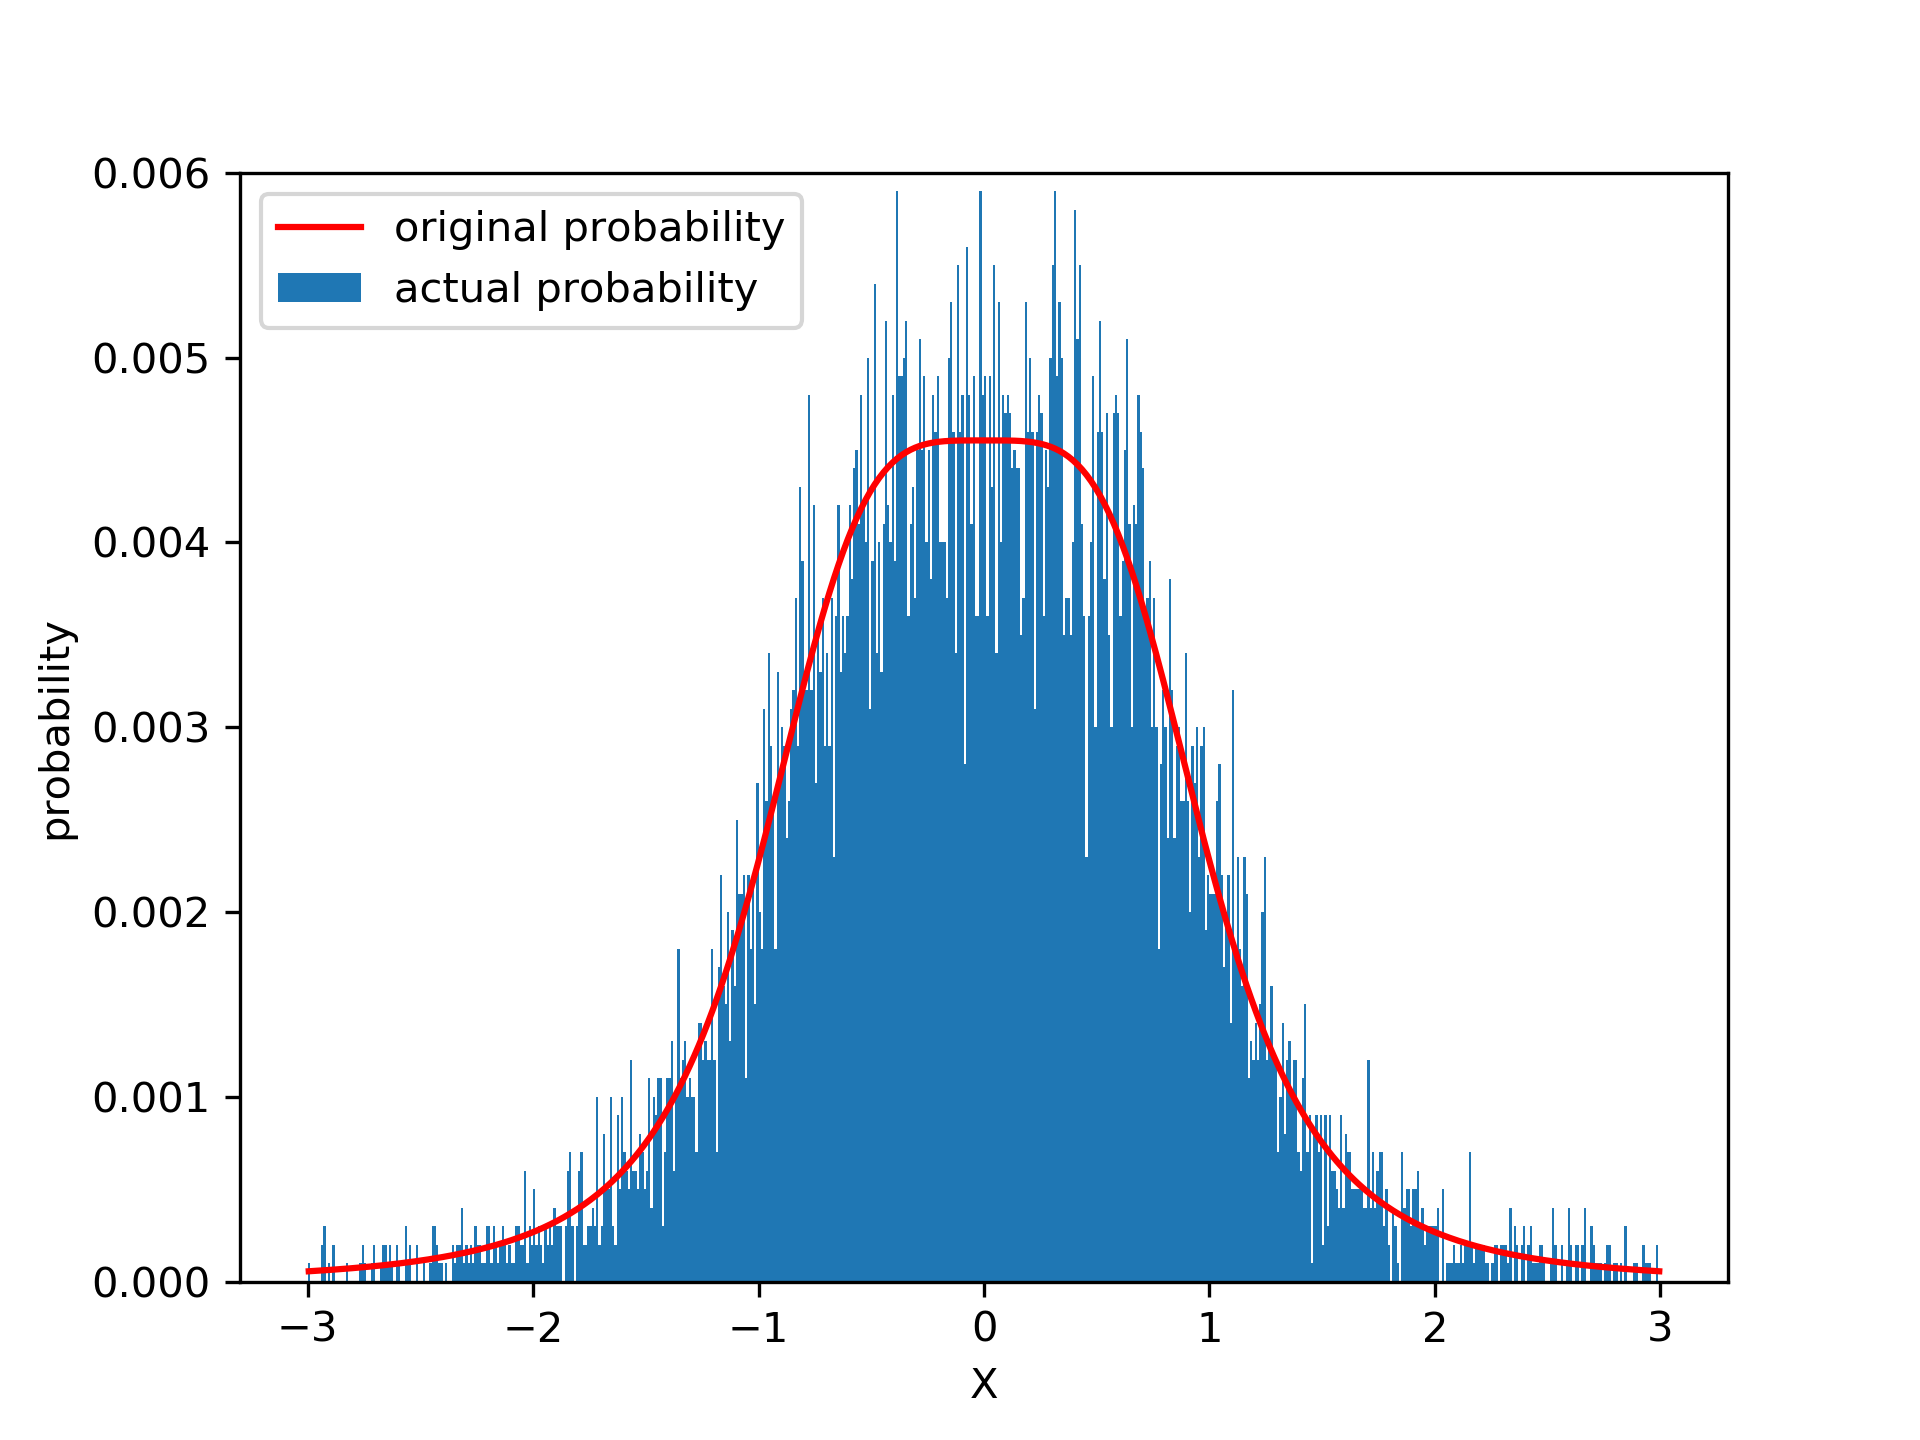
\includegraphics[width=10cm]{104.png}      
\caption{ 产生$10^{4}$个点时的结果}      
\end{figure}

\begin{figure}[!htbp]        
\centering
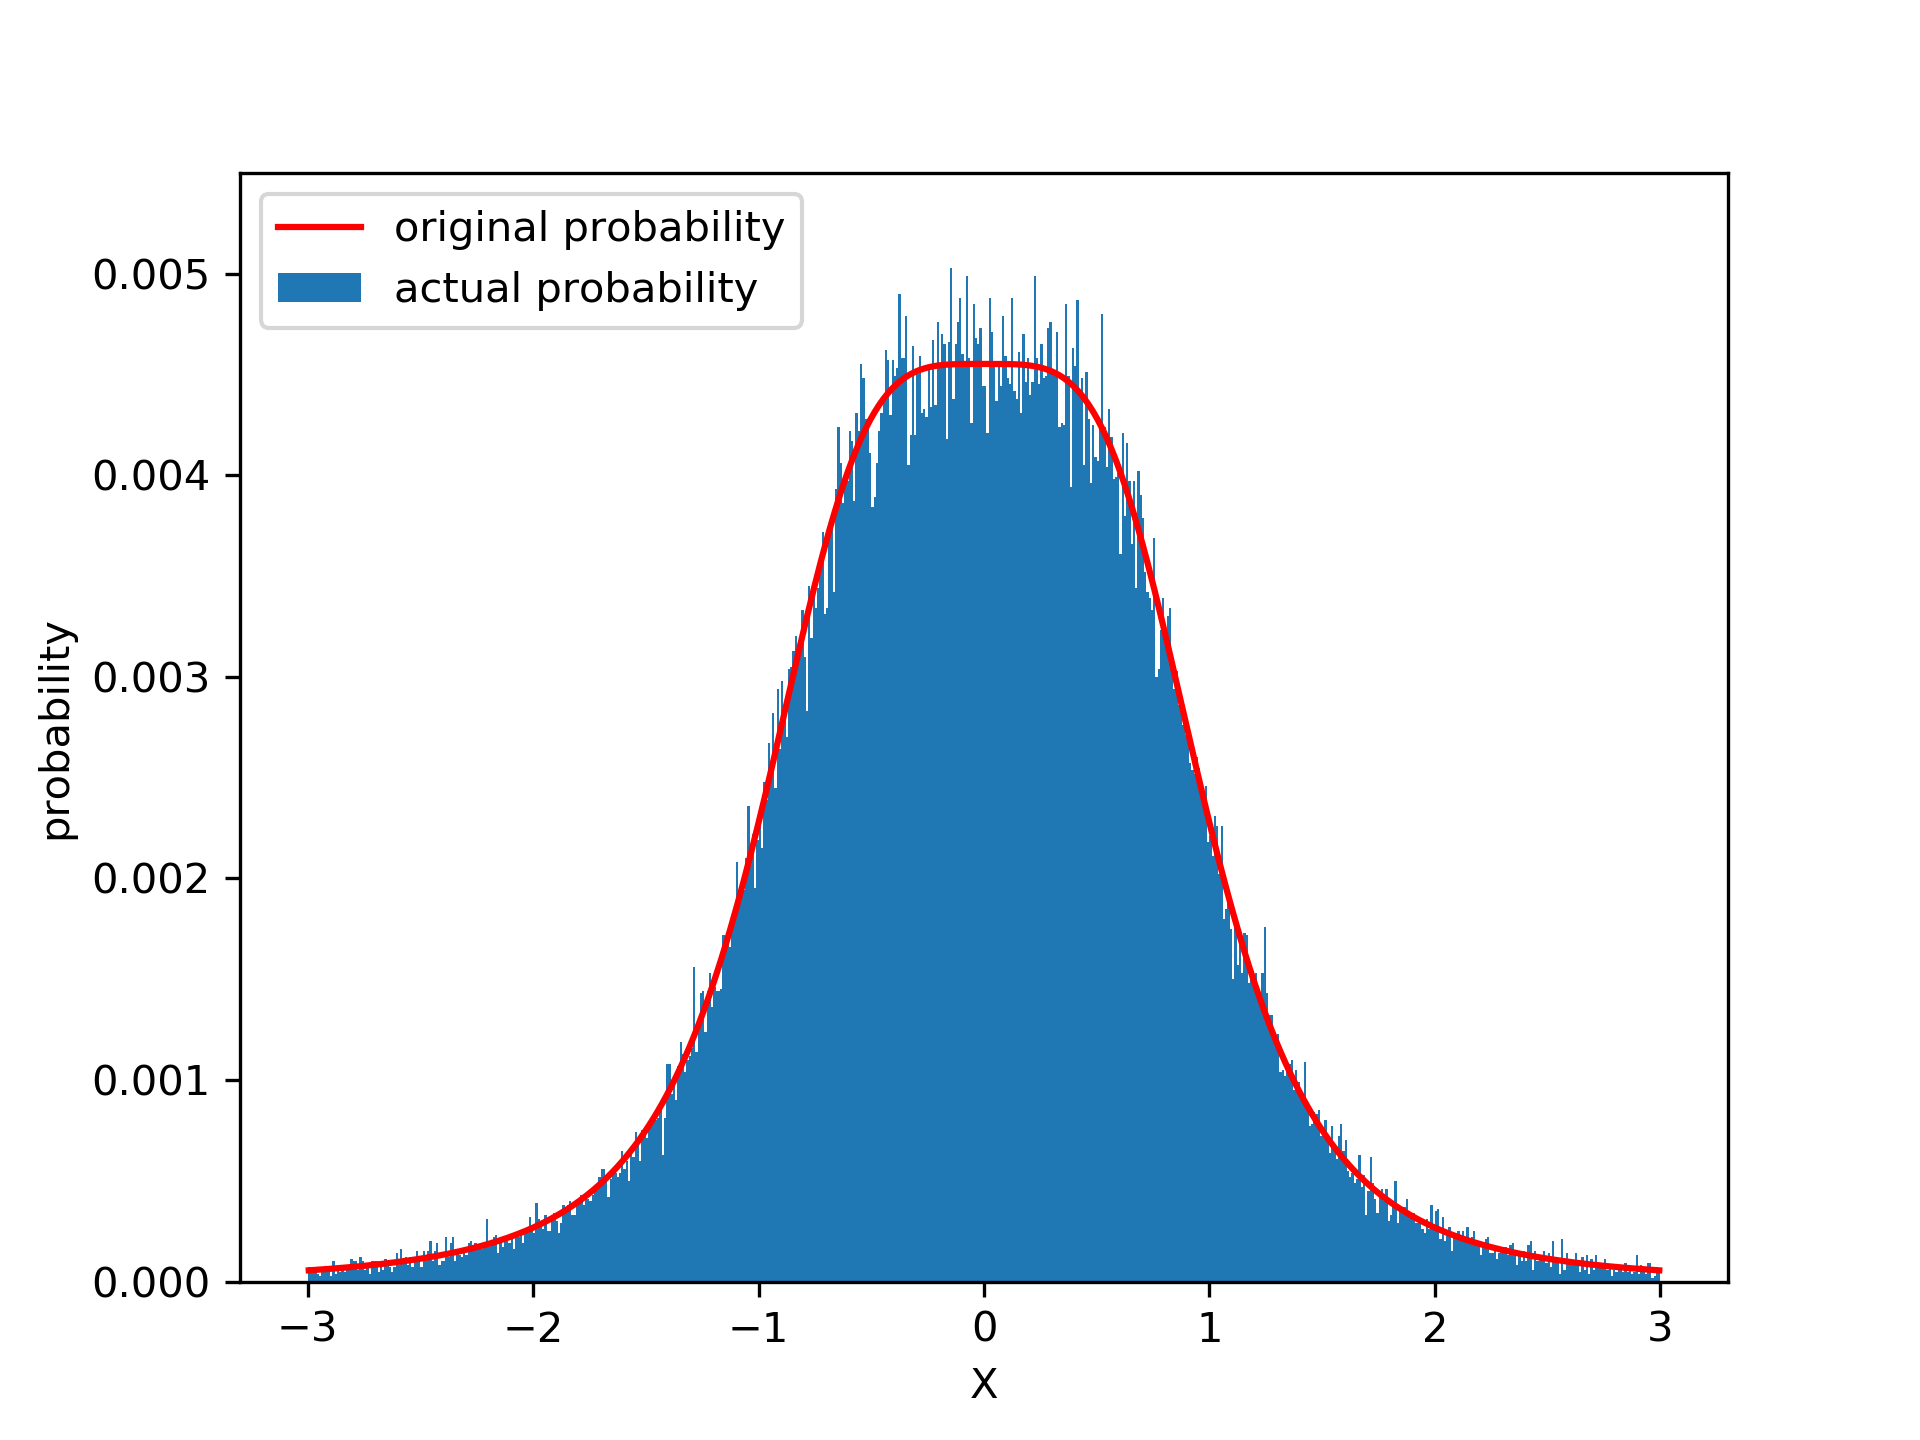
\includegraphics[width=10cm]{105.png}      
\caption{ 产生$10^{5}$个点时的结果}      
\end{figure}

\begin{figure}[!htbp]        
\centering
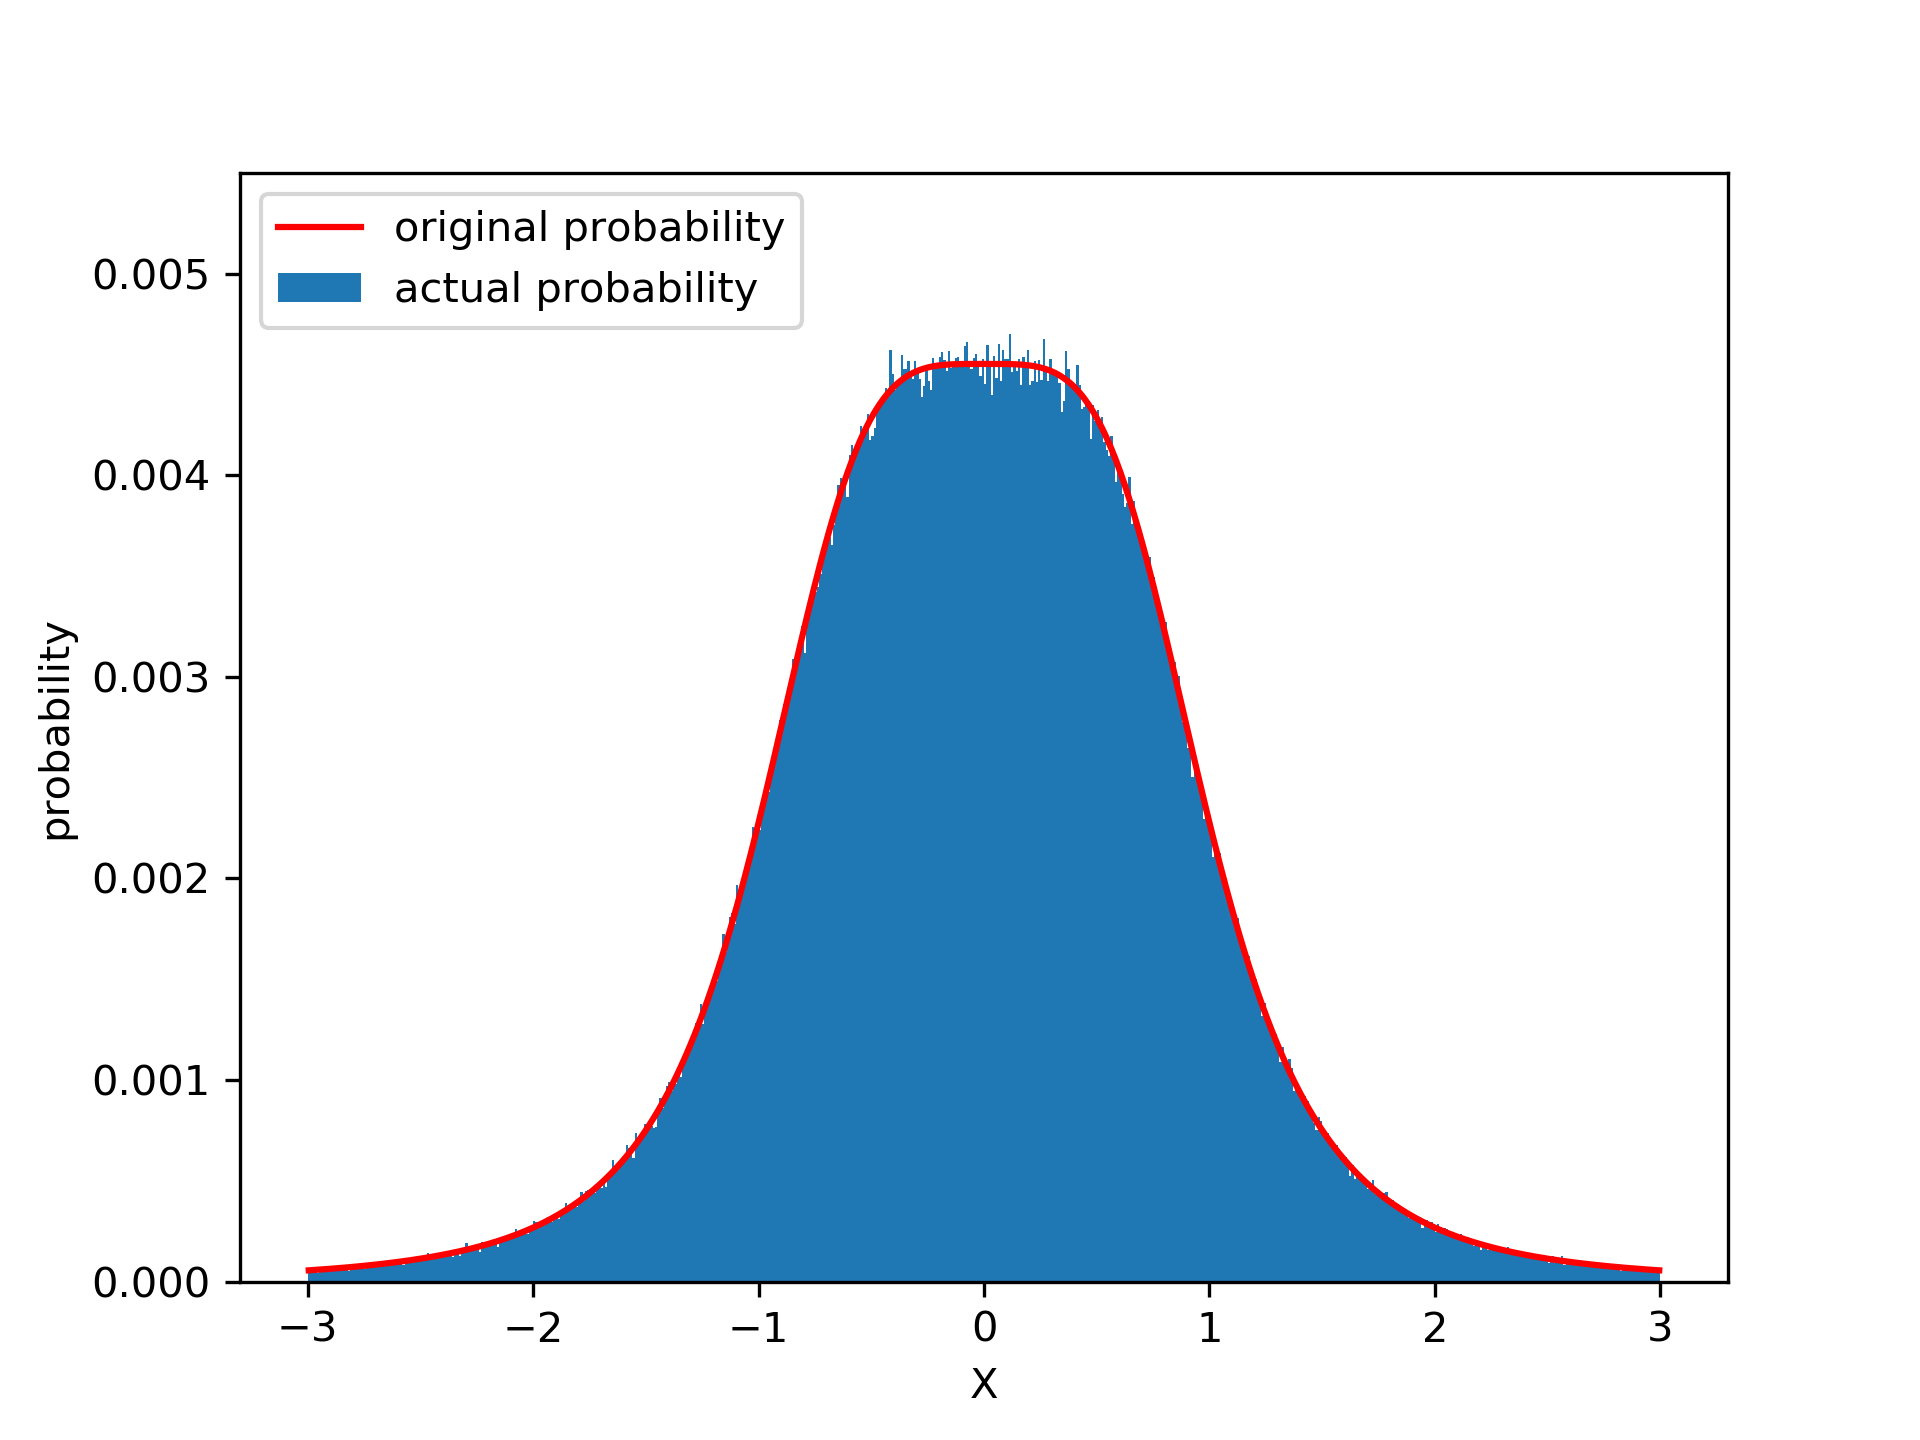
\includegraphics[width=10cm]{106.png}      
\caption{ 产生$10^{6}$个点时的结果}      
\end{figure}

\begin{figure}[!htbp]        
\centering
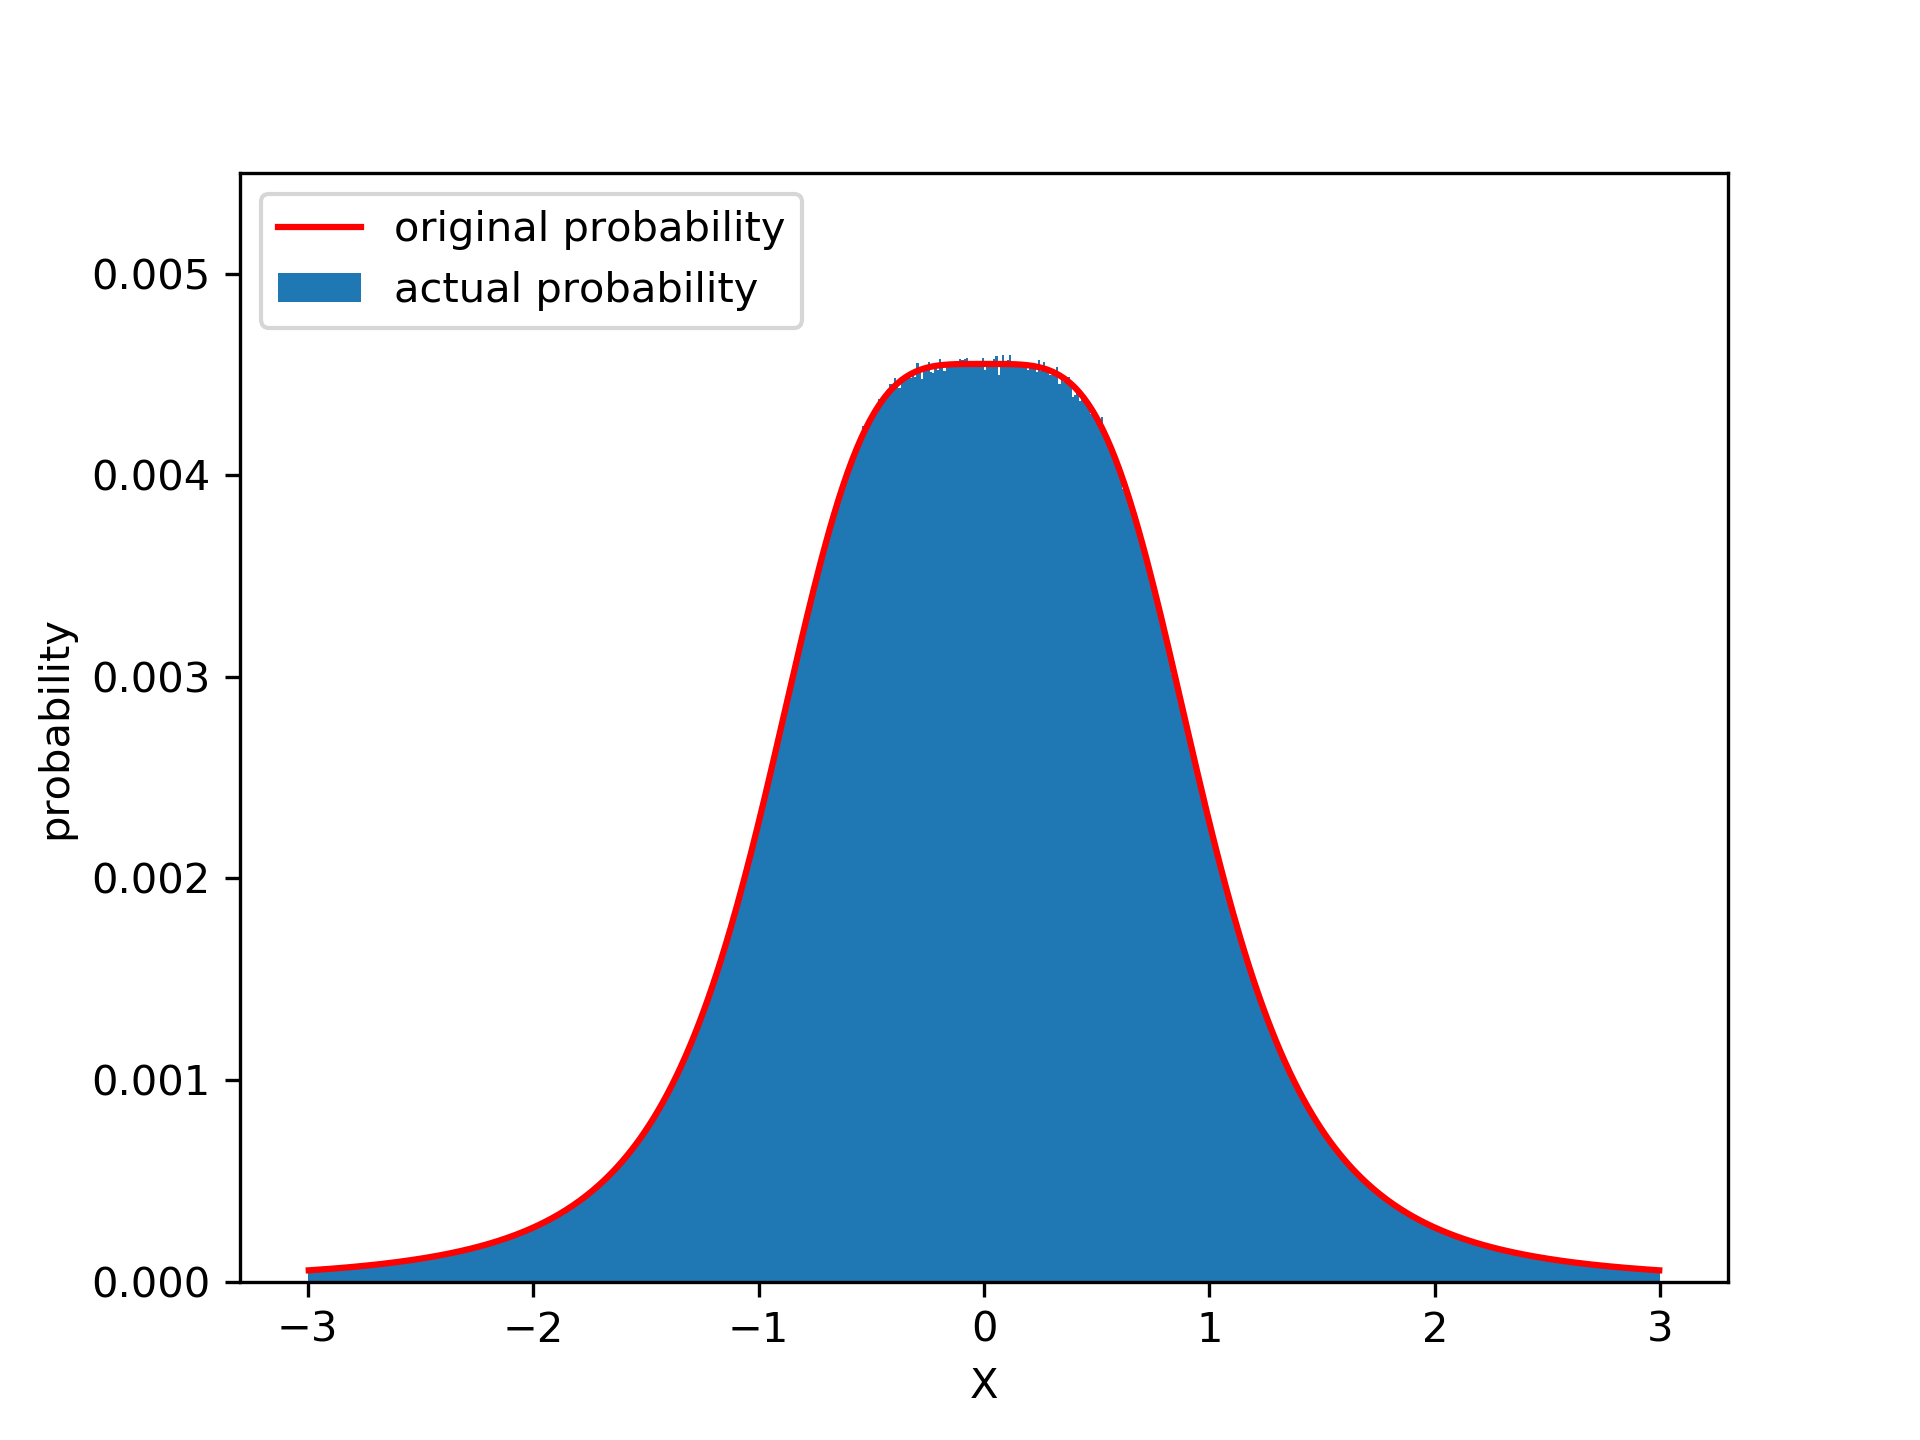
\includegraphics[width=10cm]{107.png}      
\caption{ 产生$10^{7}$个点时的结果}      
\end{figure}

\begin{figure}[!htbp]        
\centering
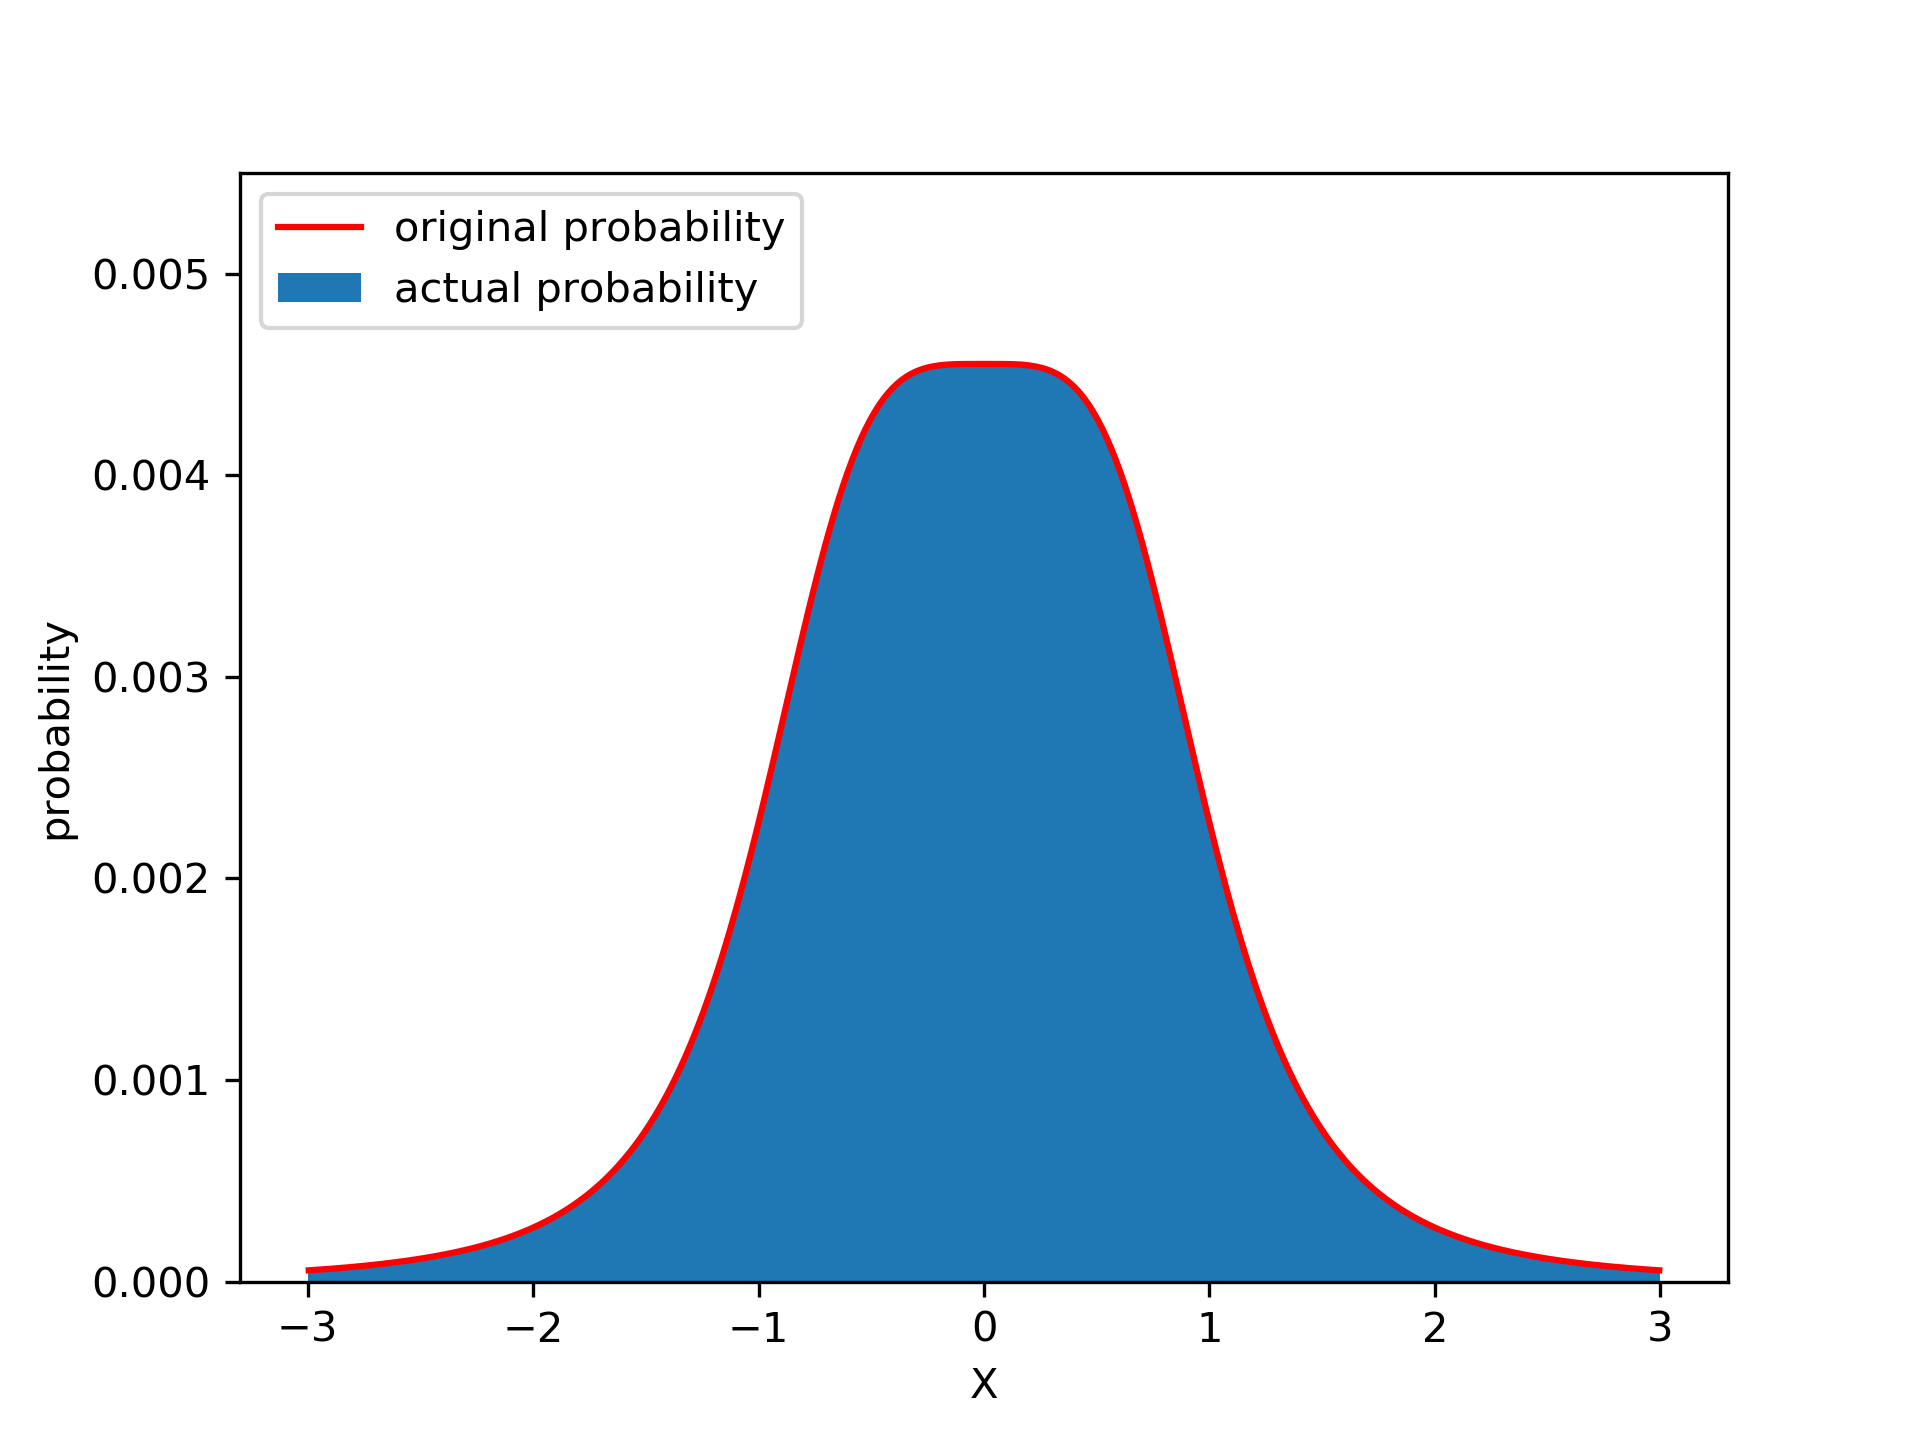
\includegraphics[width=10cm]{108.png}      
\caption{ 产生$10^{8}$个点时的结果}      
\end{figure}



\newpage
 由上述结果可以看出当总抽样点数$N=10^{8}$时,其概率分布已基本和理论概率分布重合,说明此抽样方法是成功的。而当$N$比较小时,实际抽样得到的概率分布会有“毛刺”现象,此为统计涨落造成的,特别对于$N=10^{3}$时,能明显看出有的剖分区间内甚至没有出现抽样点,而有些区间内抽样点出现的概率甚至是理论概率的2倍左右。
 
 而对不同抽样点数的抽样效率如下:

\begin{table}[!htbp]
\centering
\resizebox{\textwidth}{!}{
\begin{tabular}{|c|c|c|c|c|c|c|}
\hline

&$N=10^{3}$  &$N=10^{4}$  &$N=10^{5}$  &$N=10^{6}$  &$N=10^{7}$
&$N=10^{8}$  \\ \hline

抽样效率 &0.781861 &0.791703 &0.797486 &0.796541 &0.796881 &0.796780 \\ \hline

\end{tabular}}
\caption{抽样效率一览表}
\end{table}

可以看出此方法的抽样效率还是蛮高的,而且对于不同的抽样点数基本稳定。




\section{心得与体会}
通过此次作业,了解了对于高斯分布,一般只需对其$3\sigma$区间抽样的约定。也更加熟悉了一般连续情形的舍选抽样方法。

通过编程作业,也更加熟悉了一些C语言和\LaTeX 。

\newpage
\section{附录}

\begin{appendices}


\section{C语言源程序}
\begin{lstlisting}[language = C]
#include <stdio.h>
#include <stdlib.h>
#include <time.h>
#include <math.h>
#define a 16807
#define b 0
#define m 2147483647
#define r (m%a)
#define q (m/a)
#define Pi 3.1415926
#define e  2.718281828
#define o 600  //统计概率所剖分区域的总数


int my_filewriter_double(char str[],double num[],int n){
    FILE * fp;
    fp = fopen(str,"w+");
    
    for(int i=0;i<n;i++)
    {
        if (i == (n-1)){
            fprintf(fp,"%lf",num[i]);
            break;
        }
        fprintf(fp,"%lf,",num[i]);
        
    }
    fclose(fp);
    return 0;
}

int my_filewriter_int(char str[],int num[],int n){
    FILE * fp;
    fp = fopen(str,"w+");
    
    for(int i=0;i<n;i++)
    {
        if (i == (n-1)){
            fprintf(fp,"%d",num[i]);
            break;
        }
        fprintf(fp,"%d,",num[i]);
        
    }
    fclose(fp);
    return 0;
}



// 舍选法抽样
int  my_choose(int seed[], double ran[], int n){
    double x;
    double y;
    double u,v;
    int flag = 0;  //记录总抽样次数
    for (int j = 0; j <= n; ) {
        flag++;
        if (seed[0] >= 0) {   //产生在[0,2,4199]间均匀抽取的\xi
            u = (seed[0] / (double)m) ;
        }
        else{
            u = ((seed[0] + m) / (double)m) ;
        }
        
        if (seed[1] >= 0) {   //产生在[0,1]间均匀抽取的\eta
            v =  2*Pi*(seed[1] / (double)m);
        }
        else{
            v =   2*Pi*((seed[1] + m) / (double)m);
        }
        if (seed[2] >= 0) {   //产生在[0,1]间均匀抽取的\eta
            y =  (seed[2] / (double)m);
        }
        else{
            y =   ((seed[2] + m) / (double)m);
        }
        
        
        x = sqrt(-2*log(u))*cos(v);
        
        if( x <= 3 && x >=-3 && y*1.1*pow(e,-x*x/2) <= (1/(1+pow(x,4))) ){ //舍选条件判断
            ran[j] = x;
            j++;
        }//满足舍选法条件后写入数据

        for(int k = 0;k<3;k++){
            if(seed[k] == m-1){
                if(a >=  b){    //由于Schrage方法只对z in (0,m-1)成立,故这里要讨论z == m-1的情况
                    seed[k] = m + (b-a) % m;
                }
                else   seed[k] =  (b-a) % m;
            }
            seed[k] = ((a * (seed[k] % q) - r * (seed[k] /  q)) + b % m ) % m;
        }
    }
    
    return flag;
}




int main() {
    int N;
    int flag; //记录舍选法抽样总次数
    double p[o]; //记录在每(6/o)长度的区间内点出现的概率
    
    char str[50];
    printf("请输入您所需要的总点数:");
    while (!scanf("%d",&N)) {   //简单的输入检查,此时N变为需要产生的随机点的总数
        gets(str);
        printf("\nInput error,please try again\n");
        printf("请输入您所需要的总点数:");
    }
    if(N >1000000) printf("您输入的参数已接受,正在计算请稍等片刻~\n");
    for(int i = 0;i<o;i++){ //数组初始化
        p[i] = 0;
    }

    int seed[3] = {809576131,-1025892587,558213681}; //设置随机数产生器的初始种子值
    double *ran = malloc(sizeof(double) * N);  //用来存放舍选法产生的随机数
    
    flag = my_choose(seed, ran, N); //舍选法抽样
    
    printf("抽样效率为:%lf\n",(double)N/flag);
    int j;
    for(int i = 0;i<N;i++){  //对抽样点在每一剖分区间内出现概率进行计算
        j = (int)floor((ran[i]+3)/6*o);
        p[j] += (double)1/N;
    }
    my_filewriter_double("p.txt", p, o);  //输出抽样点在每一剖分区间内出现概率至文件

    return 0;
}

\end{lstlisting}

\newpage

\section{可视化绘图python程序源码}

\begin{lstlisting}[language = python]

import matplotlib.pyplot as plt
from mpl_toolkits.mplot3d import Axes3D
import numpy as np
#from IPython.core.pylabtools import figsize # import figsize
#figsize(12.5, 4) # 设置 figsize
plt.rcParams['savefig.dpi'] = 300 #图片像素
plt.rcParams['figure.dpi'] = 300 #分辨率
# 默认的像素:[6.0,4.0],分辨率为100,图片尺寸为 600&400
fig = plt.figure()
ax1 = fig.add_subplot(111)
X = []
Y = []

with open('problem 6/p_108.txt', 'r') as f:
    while True:
        lines = f.readline() # 整行读取数据
        if not lines:
            break
        Y = [float(i) for i in lines.split(',')]  # 将整行数据分割处理
    Y = np.array(Y) # 将数据从list类型转换为array类型。


X = np.arange(-2.995, 3.005, 0.01)

plt.bar(x=X, height=Y, width=0.01, label='actual probability')
ax1.legend(loc=1)
ax1.set_ylabel('probability')


X = np.arange(-2.995, 3.005, 0.01)
oY = 0.01/(1+X**4)/2.196879736
ax1.plot(X, oY, 'r', label='original probability')
ax1.legend(loc=2)
plt.ylim([0,0.0055])
plt.xlabel('X')


plt.savefig("2.png")

\end{lstlisting}


\end{appendices}




\end{document}
